\documentclass[12pt,a4paper, oneside]{article}
\usepackage[utf8]{inputenc}
\usepackage[T1]{fontenc}
\usepackage[english,german]{babel}
\usepackage[style=german]{csquotes}
\usepackage{graphicx}

\author{Uni Oldenburg, SWP2020 Gruppe A}

\begin{document}

    \begin{titlepage}
        \pagestyle{empty}
        \begin{center}

            \begin{figure}[h]
                \centering
                
\includegraphics[width=0.35\textwidth]{img/Logo.jpg}
            \end{figure}

            \bigskip \bigskip \noindent
            \textsc{\textbf{\LARGE Softwareprojekt:}} \par \bigskip \noindent
            \textsc{\textbf{\LARGE Projekttagebuch}}


            \par \bigskip \bigskip \bigskip \bigskip \bigskip \noindent
            {\Large Gruppe A} \par \medskip \noindent

            \par \bigskip \bigskip \bigskip \bigskip \bigskip \bigskip \noindent
            \textit{\Large Wintersemester 2020/21 und} \par \noindent
            \textit{\Large Sommersemester 2021}

            \par \bigskip \bigskip \bigskip \bigskip \bigskip \bigskip \noindent
            \par \bigskip \bigskip \bigskip \noindent
            {\Large Sprintanalyse} \par \medskip \noindent

        \end{center}
    \end{titlepage}

    \tableofcontents
    \pagebreak


    \section{Sprinttagebuch: Sprint-Nr. 1}
    \underline{Name des Sprints:}
    \\
    Golden Wind

    \noindent
    \\
    \underline{Zeitraum des Sprints:}
    \\
    04. Februar 2021 - 16. Februar 2021

    \noindent
    \\
    \underline{Ziel des Sprints:}
    \\
    Generelles Aufräumen, Abschließen, Projektdokumentation

    \noindent
    \\
    \underline {Team:}
    \\
    Sven Ahrens, Alwin Bossert, Aldin Dervisi, Marvin Drees, Mario Fokken,
    Timo Gerken, Finn Haase, Temmo Junkhoff, Maximilian Lindner, Steven Luong, Phillip-André Suhr, Eric Vuong


    \section{Vorgänge}

    \begin{itemize}
        \item SWP2020A-121: @Injects konkretisieren und korrigieren (3 Story Points)

        \item SWP2020A-123: Löschen und Bearbeiten von Nachrichten anderer Nutzer (2 Story Points)

        \item SWP2020A-136: ANmi eine Echtzeitansicht meiner Siegpunkte haben, damit ich weiß, wie weit der Sieg entfernt ist (3 Story Points)

        \item SWP2020A-137: Setter bei Messages, Requests, Responses entfernen (2 Story Points)

        \item SWP2020A-138: ServerUserService zu IUserManagement refactoren (1 Story Point)

        \item SWP2020A-139: Fehlende Interfaces erstellen (1 Story Point)

        \item SWP2020A-141: LOG-Format anpassen     (2 Story Points)

        \item SWP2020A-142: LOG-Funktion öfter nutzen (3 Story Points)

        \item SWP2020A-143: ANmi das Programm in verschiedenen Sprachen nutzen können    (3 Story Points)

        \item SWP2020A-145: UML-Dateien in .gitignore eintragen, um versehentliche Änderungen zu verhindern    (1 Story Point)

        \item SWP2020A-150: StartSession-Button ist nach dem Start einer Session immer noch anklickbar (1 Story Point)

        \item SWP2020A-154: Readystatus wird in allen offenen Lobbys gleichzeitig überschrieben    (1 Story Point)

        \item SWP2020A-156: Spielfeldrendering und Spielfeldspeicherung überarbeiten (4 Story Points)

        \item SWP2020A-157: Projekttagebuch erstellen und Sprints 1 und 4 einstellen (Erst 11, später auf 7 Story Points geschätzt)

        \item SWP2020A-165: Einige Klassen und Methoden benötigen Doku (2 Story Points)

        \item SWP2020A-168: Wiederherstellung der Lobbymindestgröße und Überarbeitung des Layouts (2 Story Points)

        \item SWP2020A-171: Mit Java-Interface Serializable auseinandersetzen, ob leere Konstruktoren nötig sind (sind sie nicht :) )    (2 Story Points)

        \item SWP2020A-172: AEmi, dass die Nutzerverwaltung von einer MySQL-DB auf dem Uniserver als Option vorliegt (2 Story Points)

        \item SWP2020A-173: AEmi, dass Einstellungen wie H2 vs MySQL auf Server oder genutzte Sprache (siehe ClientModule) in einer Config-Datei veränderbar sind (1 Story Point)

    \end{itemize}

    \subsection{Sprinterfolg}

    \begin{figure}[h]
        \centering
        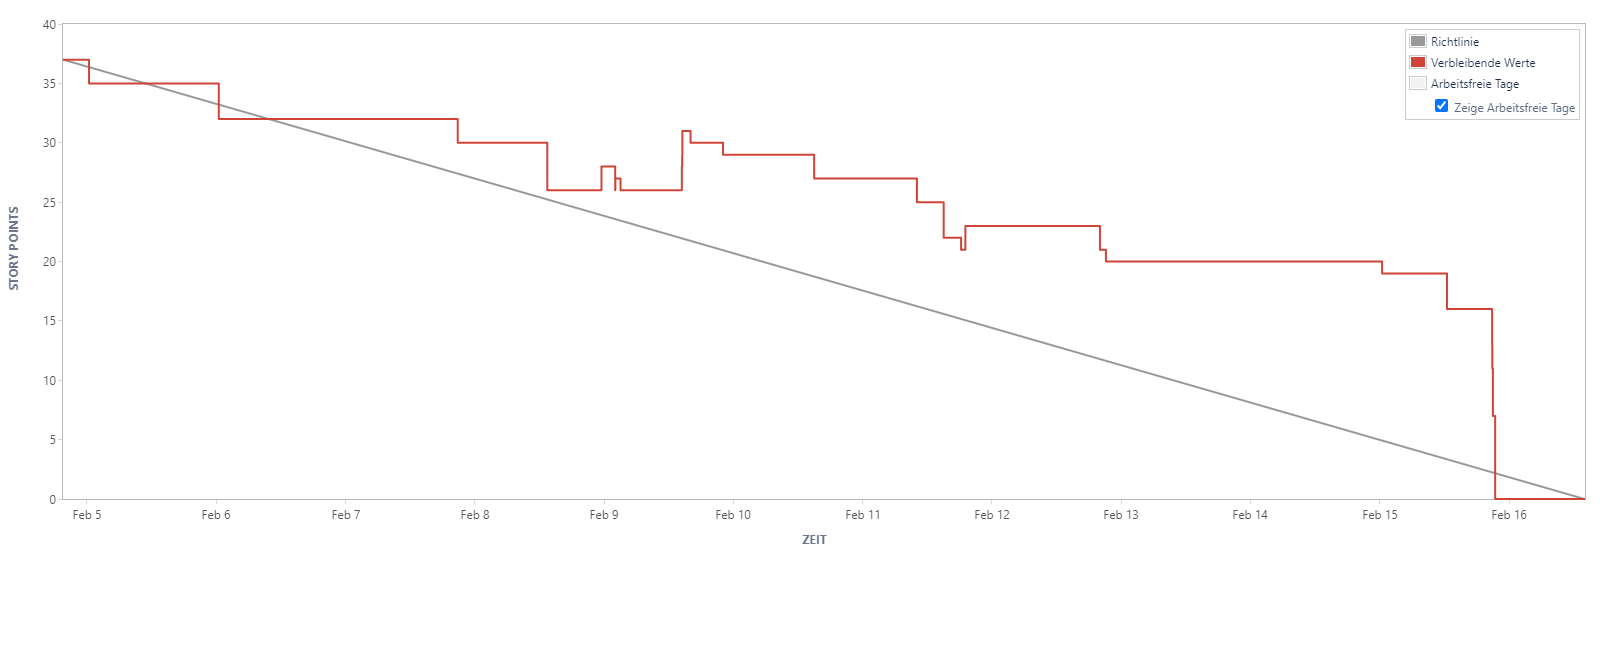
\includegraphics[width=\textwidth, height=5cm]{Burndown-Sprint 5.png}
        \caption{Burndown-Diagramm Sprint 5}
        \label{fig: Burndown-Sprint5}
    \end{figure}

    \noindent
    Am Sprintbeginn betrug der Gesamtaufwand des Sprints 37 Story Points. Während des Sprints haben wir uns entschieden, dass der Gesamtaufwand zu gering ist für einen 2 1/2 wöchigen Sprint. Daher haben wir folgende Vorgänge nachgezogen:

    \begin{itemize}
        \item SWP2020A-154: Readystatus wird in allen offenen Lobbys gleichzeitig überschrieben    (1 Story Point)

        \item SWP2020A-165: Einige Klassen und Methoden benötigen Doku (2 Story Points)

        \item SWP2020A-168: Wiederherstellung der Lobbymindestgröße und Überarbeitung des Layouts (2 Story Points)

        \item SWP2020A-171: Mit Java-Interface Serializable auseinandersetzen, ob leere Konstruktoren nötig sind (sind sie nicht :) )    (2 Story Points)

        \item SWP2020A-172: AEmi, dass die Nutzerverwaltung von einer MySQL-DB auf dem Uniserver als Option vorliegt (2 Story Points)


        \item SWP2020A-173: AEmi, dass Einstellungen wie H2 vs MySQL auf Server oder genutzte Sprache (siehe ClientModule) in einer Config-Datei veränderbar sind (1 Story Point)

    \end{itemize}

    \noindent
    Im Burndown-Diagramm wird erkenntlich, dass viele Vorgänge bereits frühzeitig abgeschlossen wurden. Deswegen wurden mehrere Vorgänge nachgezogen, da viele vorzeitig mit ihren Tasks und Reviews fertig waren und somit über mehr als der Hälfte des Sprintzeitraums keine Vorgänge mehr hätten. Des Weiteren wurde der Sprint frühzeitig beendet, da bereits alle Vorgänge beendet wurden. Somit wurden 43 Story-Points erreicht von den am Sprintbeginn geplanten 37 Story-Points.

    \subsection{Sprintprobleme bzw. Hindernisse}
    Es gab hinsichtlich bei den zu bearbeitenden Vorgängen keine direkten Probleme, wobei jedoch im Burndown-Diagramm zu erkennen ist, dass der Sprintumfang nicht optimal durchdacht wurde.
    \noindent
    Schließlich mussten zahlreiche Vorgänge nachgezogen werden und der Sprintzeitraum wurde sogar um 3 Tage verringert.


    \section{Erkenntnis aus der Retrospektive}
    Folgende Erkenntnisse ergaben sich aus der Retrospektive:\\

    \underline{Start}
    \begin{itemize}
        \item Hilfsbereitschaft aufrechterhalten
        \item Ideen in den Backlog werfen
        \item Bugs in den Backlog werfen
        \item Pair-Programming beibehalten
        \\
    \end{itemize}

    \underline{Stop}
    \begin{itemize}
        \item Review nach max. 48 Stunden nach PR fertig haben
        \item Anfangen mit Bearbeitung in den ersten paar Tagen des Sprints
        \\
    \end{itemize}

    \underline{Weiter so}
    \begin{itemize}
        \item Bei akutem Arbeitsmangel Vorgänge nachziehen
        \item Sprecht euch ab
        \item Features Testen
        \item Auch andere Features auf Kollateralschaden prüfen
        \item Ausfürliche Commitnachrichten beibehalten
        \\
    \end{itemize}


    \section{Fazit}
    Der fünfte Sprint war der erste im SWP2020A, welchen wir sowohl um weitere Vorgänge erweitert als auch den Sprintzeitraum gekürzt haben. Er wurde anfangs so klein gehalten, da wir uns außerhalb des Projekts mitten in der Klausurenphase befanden und wir einen kleineren Sprint für sinnvoll hielten. Jedoch hat sich gezeigt, dass trotz Klausurenstress wir unsere Vorgänge zügig und frühzeitig fertig gestellt haben und somit der Sprintumfang erweitert werden konnte.
    Wir haben uns für folgende Sprints vorgenommen, dass wir den Umfang der Sprints nicht mehr als Final betrachten, sondern auch um weitere Vorgänge erweitern können, falls Vorgänge frühzeitig beendet werden und somit einzelne Teammitglieder für den restlichen Sprintzeitraum keine Arbeit mehr haben.
    Dazu möchten wir unsere Reviews bzw. Tests ausführlicher durchführen, um Fehler und Mergekonflikte frühzeitig erkennen zu können.
    Weiterhin sollen alle Teammitglieder aktiv dazu beitragen, Ideen und eventuelle Bugfixes regelmäßig in den Backlog hinzuzufügen.

\end{document}
